\documentclass[10pt, aspectratio=169]{beamer}

% === TEMA ===
\usetheme{Madrid}
\usecolortheme{default}
\setbeamertemplate{footline}{}
\setbeamertemplate{navigation symbols}{}

% === PAKET TAMBAHAN ===
\usepackage[utf8]{inputenc}
\usepackage{graphicx}
\usepackage{hyperref}
\usepackage{booktabs}
\usepackage{multirow}
\usepackage{array}
\usepackage{xcolor}
\usepackage{listings}
\usepackage{tikz}
\usetikzlibrary{arrows.meta, positioning, shapes.geometric, fit}

% === PENGATURAN WARNA ===
\definecolor{mainblue}{RGB}{0, 102, 204}
\definecolor{lightblue}{RGB}{230, 242, 255}
\definecolor{darkblue}{RGB}{0, 51, 102}

\setbeamercolor{titlelike}{bg=mainblue, fg=white}
\setbeamercolor{frametitle}{bg=mainblue, fg=white}
\setbeamercolor{structure}{fg=mainblue}
\setbeamercolor{block title}{bg=mainblue, fg=white}
\setbeamercolor{block body}{bg=lightblue, fg=black}

% === INFORMASI DOKUMEN ===
\title{Aplikasi Obibi: Pengingat Jadwal Obat Pintar}
\subtitle{Presentasi SKPL, DPPL, \& DUPL}
\author{Najla Tsabita Afiyah \and Revalina Rasyidin \and Ravi Adi Prakoso \and Muhammad Ahsan Raziq Sulthany}
\institute[Universitas Telkom]{\small Program Studi S1 Informatika\\Fakultas Informatika\\Universitas Telkom}
\date{2026}

% === AWAL DOKUMEN ===
\begin{document}

% --- SLIDE JUDUL ---
\begin{frame}
    \titlepage
    \begin{center}
        \tiny{Dosen Pengampu: Helmi Faisal Muttaqin, S.Kom., M.T.}
    \end{center}
\end{frame}

% --- DAFTAR ISI ---
\begin{frame}{Daftar Isi}
    \tableofcontents
\end{frame}

% ======================================================================
% BAGIAN 1: PENDAHULUAN & GAMBARAN UMUM
% ======================================================================
\section{Pendahuluan \& Gambaran Umum}

% --- SLIDE: LATAR BELAKANG ---
\begin{frame}{Latar Belakang}
    \begin{itemize}
        \item Banyak pasien kronis, lansia, dan penyandang disabilitas kesulitan mengikuti jadwal pengobatan.
        \item Keterbatasan fisik, kognitif, dan akses teknologi menjadi kendala utama.
        \item Dibutuhkan solusi digital yang \textbf{inklusif, mudah digunakan, dan cerdas}.
    \end{itemize}
    \vspace{0.5cm}
    \begin{block}{Solusi: Aplikasi Obibi}
        Asisten kesehatan berbasis \textbf{Agentic AI} dan \textbf{GraphRAG} untuk:
        \begin{itemize}
            \item Pengingat obat otomatis dan personal.
            \item Analisis interaksi antar obat secara mandiri.
            \item Chatbot AI dengan dukungan perintah suara.
        \end{itemize}
    \end{block}
\end{frame}

% --- SLIDE: TUJUAN PRODUK ---
\begin{frame}{Tujuan \& Manfaat Produk}
    \begin{columns}[T]
        \column{0.5\textwidth}
        \textbf{Tujuan Utama:}
        \begin{itemize}
            \item Meningkatkan kepatuhan pasien terhadap pengobatan.
            \item Menyediakan pengingat yang terpersonalisasi dan inklusif.
            \item Memberikan akses informasi kesehatan yang aman dan akurat.
        \end{itemize}
        
        \column{0.5\textwidth}
        \textbf{Manfaat:}
        \begin{itemize}
            \item \textbf{Pasien}: Pengingat otomatis, asisten virtual 24/7.
            \item \textbf{Tenaga Medis}: Membantu memantau kepatuhan pasien.
            \item \textbf{Ekosistem Kesehatan}: Model sistem kesehatan inklusif berbasis AI.
        \end{itemize}
    \end{columns}
\end{frame}

% --- SLIDE: PROFIL PENGGUNA ---
\begin{frame}{Profil \& Kelas Pengguna}
    \begin{itemize}
        \item \textbf{Pasien (Utama)}:
        \begin{itemize}
            \item Lansia dan penyandang disabilitas.
            \item Pasien kronis dengan pengobatan rutin.
            \item Kemampuan teknis rendah hingga menengah.
        \end{itemize}
        \item \textbf{Medical Admin / Apoteker (Sekunder)}:
        \begin{itemize}
            \item Mengelola \textit{Knowledge Base} obat dan interaksi.
            \item Memutakhirkan data medis berdasarkan literatur terbaru.
        \end{itemize}
    \end{itemize}
\end{frame}

% ======================================================================
% BAGIAN 2: KEBUTUHAN PERANGKAT LUNAK (SKPL)
% ======================================================================
\section{Spesifikasi Kebutuhan Perangkat Lunak}

% --- SLIDE: KEBUTUHAN FUNGSIONAL (FR) ---
\begin{frame}{Kebutuhan Fungsional (FR)}
    \begin{table}[]
    \tiny
    \begin{tabular}{|c|c|p{0.45\textwidth}|c|}
        \hline
        \textbf{No} & \textbf{Kode FR} & \textbf{Nama Fungsional} & \textbf{Tipe FR} \\
        \hline
        1 & FR-01 & Autentikasi Pengguna (Login/Register) & Must Have \\
        2 & FR-02 & Manajemen Data Obat & Must Have \\
        3 & FR-03 & Penjadwalan Konsumsi Obat & Must Have \\
        4 & FR-04 & Notifikasi Pengingat Obat & Must Have \\
        5 & FR-05 & Pencatatan Kepatuhan Konsumsi & Must Have \\
        6 & FR-06 & Laporan \& Ekspor Kepatuhan & Satisfy \\
        7 & FR-07 & Konsultasi AI Assistant & Must Have \\
        8 & FR-08 & Penambahan Obat Otomatis via AI & Satisfy \\
        9 & FR-09 & Konversi Suara ke Teks (STT) & Delighter \\
        10 & FR-10 & Deteksi Interaksi Antarobat & Must Have \\
        \hline
    \end{tabular}
    \end{table}
    \vspace{0.1cm}
    \begin{flushright}
        \tiny{\textit{Sumber: SKPL Aplikasi Obibi}}
    \end{flushright}
\end{frame}

% --- SLIDE: KEBUTUHAN NON-FUNGSIONAL (NFR) ---
\begin{frame}{Kebutuhan Non-Fungsional (NFR)}
    \begin{table}[]
    \tiny
    \begin{tabular}{|c|p{0.4\textwidth}|c|}
        \hline
        \textbf{No} & \textbf{Kriteria Kualitas} & \textbf{Kode} \\
        \hline
        1 & \textbf{Usability}: SUS minimal 80, ramah lansia/disabilitas & NFR-01 \\
        2 & \textbf{Reliability}: Uptime 99\%, pengingat tetap jalan meski offline & NFR-02 \\
        3 & \textbf{Performance}: Loading < 3 detik, AI < 10 detik & NFR-03 \\
        4 & \textbf{Security}: Enkripsi AES-256, OAuth 2.0 & NFR-04 \\
        5 & \textbf{Availability}: 24/7, fallback mechanism & NFR-05 \\
        6 & \textbf{Maintainability}: Arsitektur modular & NFR-06 \\
        7 & \textbf{Scalability}: 10.000 pengguna aktif harian & NFR-07 \\
        8 & \textbf{Portability}: Android ≥ v8.0, iOS ≥ v12 & NFR-08 \\
        9 & \textbf{Accessibility}: Voice interaction, screen reader & NFR-09 \\
        10 & \textbf{Compliance}: UU PDP, ISO 27001 & NFR-10 \\
        \hline
    \end{tabular}
    \end{table}
\end{frame}

% ======================================================================
% BAGIAN 3: PERANCANGAN PERANGKAT LUNAK (DPPL)
% ======================================================================
\section{Perancangan Perangkat Lunak}

% --- SLIDE: ARSITEKTUR SISTEM ---
\begin{frame}{Arsitektur Perangkat Lunak}
    \centering
    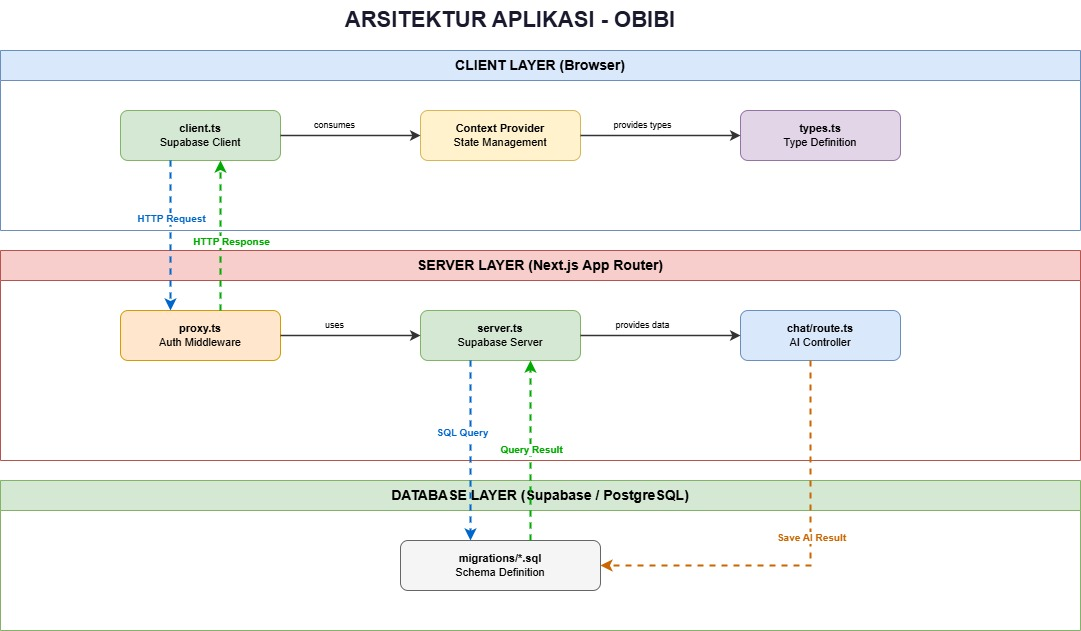
\includegraphics[height=0.55\textheight, keepaspectratio]{arsitektur.jpeg}
    \begin{flushright}
        \tiny{\textit{Sumber: DPPL Aplikasi Obibi}}
    \end{flushright}
\end{frame}

% --- SLIDE: USE CASE DIAGRAM ---
\begin{frame}{Use Case Diagram}
    \centering
    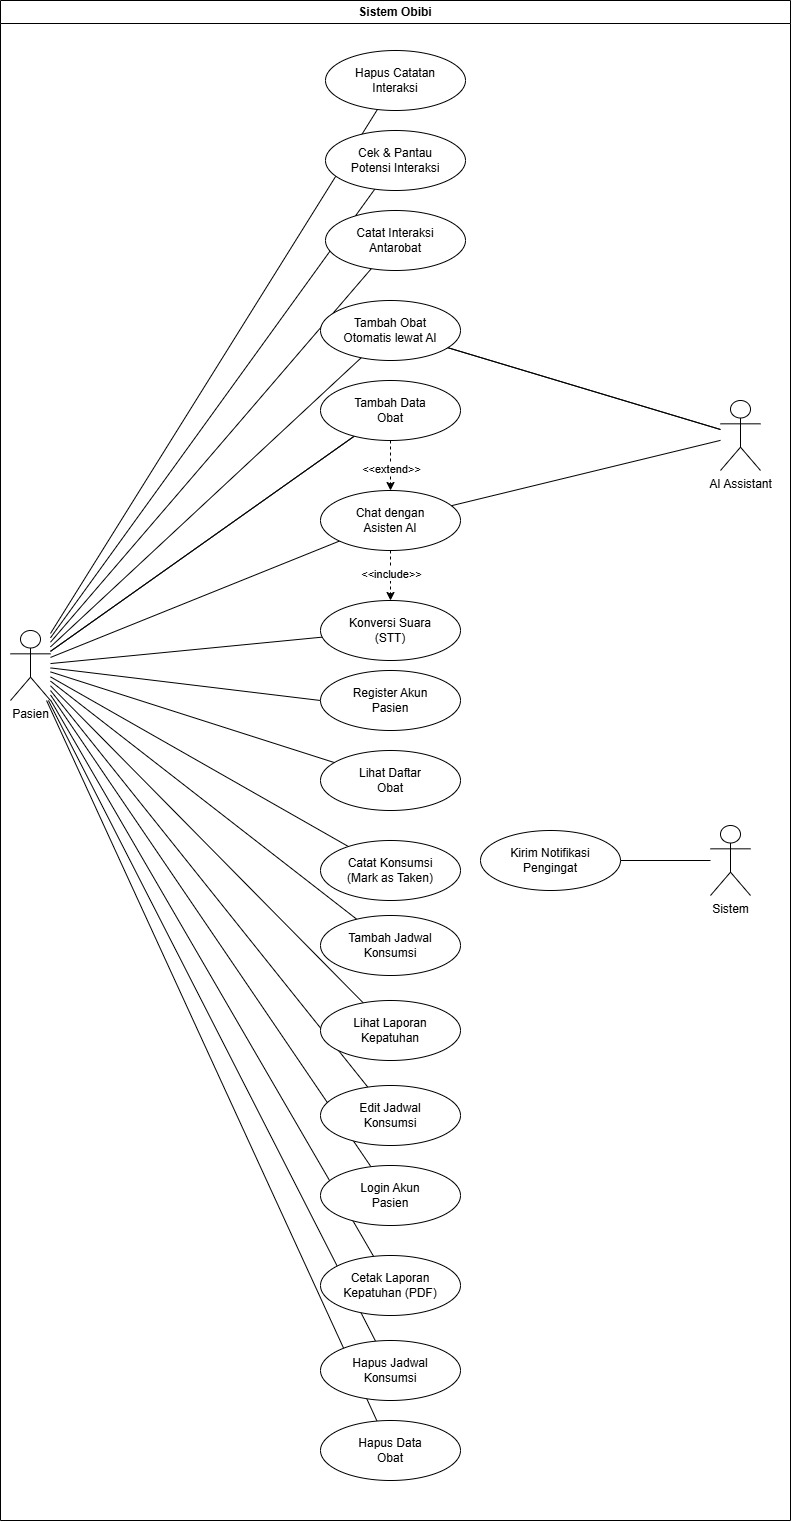
\includegraphics[height=0.55\textheight, keepaspectratio]{usecase.jpeg}
    \begin{flushright}
        \tiny{\textit{Sumber: DPPL Aplikasi Obibi}}
    \end{flushright}
\end{frame}

% --- SLIDE: ERD ---
\begin{frame}{Entity Relationship Diagram (ERD)}
    \centering
    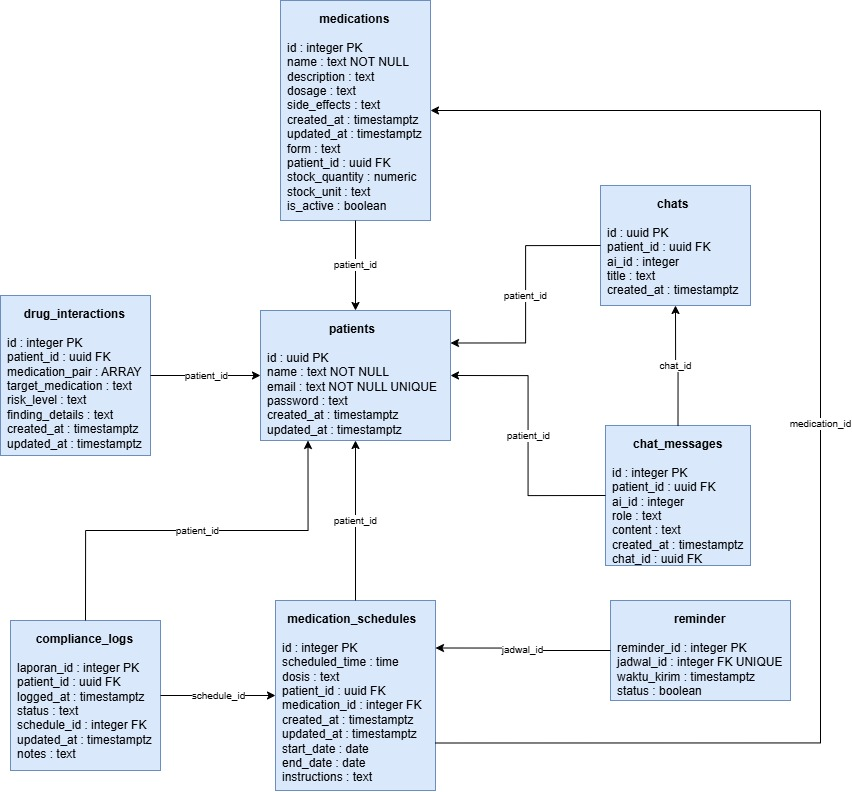
\includegraphics[height=0.55\textheight, keepaspectratio]{erd.jpeg}
    \begin{flushright}
        \tiny{\textit{Sumber: SKPL \& DPPL Aplikasi Obibi}}
    \end{flushright}
\end{frame}

% --- SLIDE: DIAGRAM KELAS ---
\begin{frame}{Diagram Kelas (Perancangan)}
    \centering
    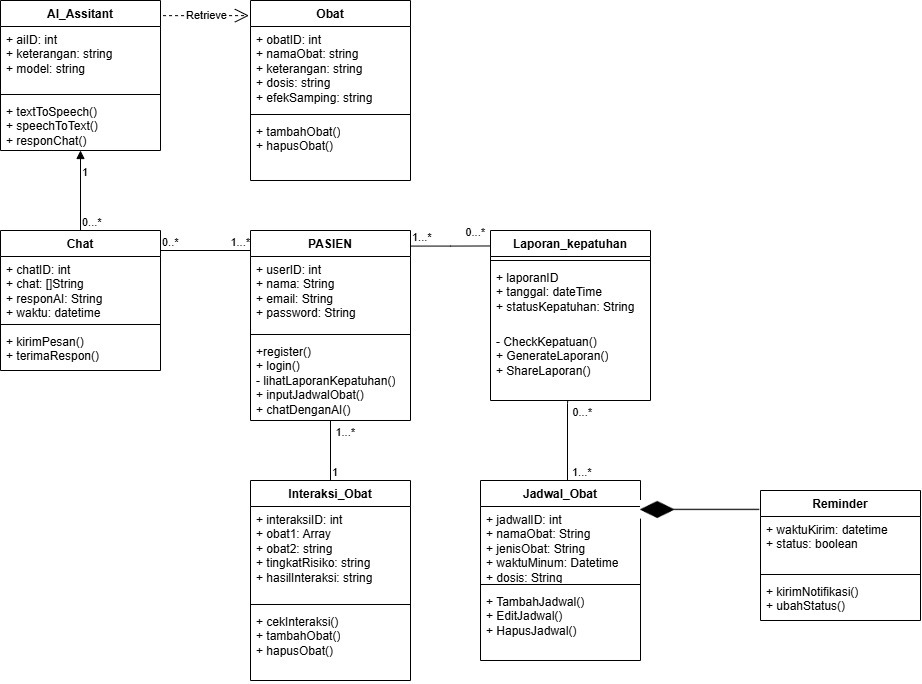
\includegraphics[height=0.55\textheight, keepaspectratio]{class_diagram.jpeg}
    \begin{flushright}
        \tiny{\textit{Sumber: DPPL Aplikasi Obibi}}
    \end{flushright}
\end{frame}

% --- SLIDE: USE CASE SCENARIO #1 ---
\begin{frame}{Use Case: Registrasi Pengguna Baru}
    \centering
    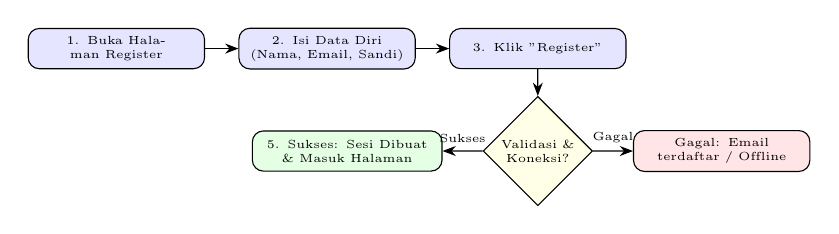
\begin{tikzpicture}[auto, >=Stealth, scale=0.85, every node/.style={transform shape},
        block/.style={rectangle, draw, fill=blue!10, text width=2.4cm, align=center, rounded corners, minimum height=0.6cm, font=\tiny},
        decision/.style={diamond, draw, fill=yellow!10, text width=1.3cm, align=center, inner sep=0pt, font=\tiny},
        err/.style={rectangle, draw, fill=red!10, text width=2.4cm, align=center, rounded corners, minimum height=0.6cm, font=\tiny},
        succ/.style={rectangle, draw, fill=green!10, text width=2.6cm, align=center, rounded corners, minimum height=0.6cm, font=\tiny}]
        
        \node (n1) [block] {1. Buka Halaman Register};
        \node (n2) [block, right=0.5cm of n1] {2. Isi Data Diri (Nama, Email, Sandi)};
        \node (n3) [block, right=0.5cm of n2] {3. Klik "Register"};
        \node (n4) [decision, below=0.4cm of n3] {Validasi \& Koneksi?};
        \node (n5) [succ, left=0.6cm of n4] {5. Sukses: Sesi Dibuat \& Masuk Halaman};
        \node (n6) [err, right=0.6cm of n4] {Gagal: Email terdaftar / Offline};
        
        \draw[->] (n1) -- (n2);
        \draw[->] (n2) -- (n3);
        \draw[->] (n3) -- (n4);
        \draw[->] (n4) -- node[above] {\tiny Sukses} (n5);
        \draw[->] (n4) -- node[above] {\tiny Gagal} (n6);
    \end{tikzpicture}
\end{frame}

% --- SLIDE: USE CASE SCENARIO #2 ---
\begin{frame}{Use Case: Login Pengguna}
    \centering
    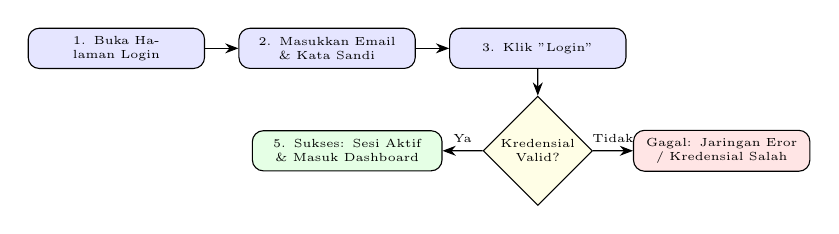
\begin{tikzpicture}[auto, >=Stealth, scale=0.85, every node/.style={transform shape},
        block/.style={rectangle, draw, fill=blue!10, text width=2.4cm, align=center, rounded corners, minimum height=0.6cm, font=\tiny},
        decision/.style={diamond, draw, fill=yellow!10, text width=1.3cm, align=center, inner sep=0pt, font=\tiny},
        err/.style={rectangle, draw, fill=red!10, text width=2.4cm, align=center, rounded corners, minimum height=0.6cm, font=\tiny},
        succ/.style={rectangle, draw, fill=green!10, text width=2.6cm, align=center, rounded corners, minimum height=0.6cm, font=\tiny}]
        
        \node (n1) [block] {1. Buka Halaman Login};
        \node (n2) [block, right=0.5cm of n1] {2. Masukkan Email \& Kata Sandi};
        \node (n3) [block, right=0.5cm of n2] {3. Klik "Login"};
        \node (n4) [decision, below=0.4cm of n3] {Kredensial Valid?};
        \node (n5) [succ, left=0.6cm of n4] {5. Sukses: Sesi Aktif \& Masuk Dashboard};
        \node (n6) [err, right=0.6cm of n4] {Gagal: Jaringan Eror / Kredensial Salah};
        
        \draw[->] (n1) -- (n2);
        \draw[->] (n2) -- (n3);
        \draw[->] (n3) -- (n4);
        \draw[->] (n4) -- node[above] {\tiny Ya} (n5);
        \draw[->] (n4) -- node[above] {\tiny Tidak} (n6);
    \end{tikzpicture}
\end{frame}

% --- SLIDE: USE CASE SCENARIO #3 ---
\begin{frame}{Use Case: Kelola Data Obat}
    \centering
    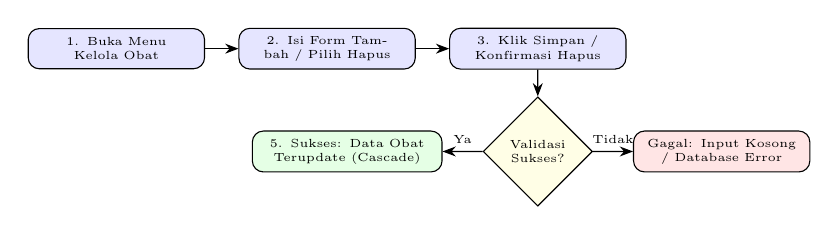
\begin{tikzpicture}[auto, >=Stealth, scale=0.85, every node/.style={transform shape},
        block/.style={rectangle, draw, fill=blue!10, text width=2.4cm, align=center, rounded corners, minimum height=0.6cm, font=\tiny},
        decision/.style={diamond, draw, fill=yellow!10, text width=1.3cm, align=center, inner sep=0pt, font=\tiny},
        err/.style={rectangle, draw, fill=red!10, text width=2.4cm, align=center, rounded corners, minimum height=0.6cm, font=\tiny},
        succ/.style={rectangle, draw, fill=green!10, text width=2.6cm, align=center, rounded corners, minimum height=0.6cm, font=\tiny}]
        
        \node (n1) [block] {1. Buka Menu Kelola Obat};
        \node (n2) [block, right=0.5cm of n1] {2. Isi Form Tambah / Pilih Hapus};
        \node (n3) [block, right=0.5cm of n2] {3. Klik Simpan / Konfirmasi Hapus};
        \node (n4) [decision, below=0.4cm of n3] {Validasi Sukses?};
        \node (n5) [succ, left=0.6cm of n4] {5. Sukses: Data Obat Terupdate (Cascade)};
        \node (n6) [err, right=0.6cm of n4] {Gagal: Input Kosong / Database Error};
        
        \draw[->] (n1) -- (n2);
        \draw[->] (n2) -- (n3);
        \draw[->] (n3) -- (n4);
        \draw[->] (n4) -- node[above] {\tiny Ya} (n5);
        \draw[->] (n4) -- node[above] {\tiny Tidak} (n6);
    \end{tikzpicture}
\end{frame}

% --- SLIDE: USE CASE SCENARIO #4 ---
\begin{frame}{Use Case: Input Jadwal Minum Obat}
    \centering
    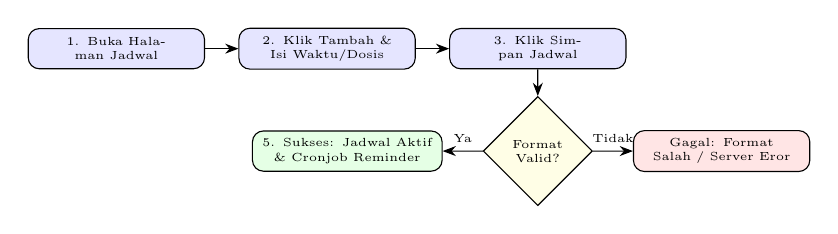
\begin{tikzpicture}[auto, >=Stealth, scale=0.85, every node/.style={transform shape},
        block/.style={rectangle, draw, fill=blue!10, text width=2.4cm, align=center, rounded corners, minimum height=0.6cm, font=\tiny},
        decision/.style={diamond, draw, fill=yellow!10, text width=1.3cm, align=center, inner sep=0pt, font=\tiny},
        err/.style={rectangle, draw, fill=red!10, text width=2.4cm, align=center, rounded corners, minimum height=0.6cm, font=\tiny},
        succ/.style={rectangle, draw, fill=green!10, text width=2.6cm, align=center, rounded corners, minimum height=0.6cm, font=\tiny}]
        
        \node (n1) [block] {1. Buka Halaman Jadwal};
        \node (n2) [block, right=0.5cm of n1] {2. Klik Tambah \& Isi Waktu/Dosis};
        \node (n3) [block, right=0.5cm of n2] {3. Klik Simpan Jadwal};
        \node (n4) [decision, below=0.4cm of n3] {Format Valid?};
        \node (n5) [succ, left=0.6cm of n4] {5. Sukses: Jadwal Aktif \& Cronjob Reminder};
        \node (n6) [err, right=0.6cm of n4] {Gagal: Format Salah / Server Eror};
        
        \draw[->] (n1) -- (n2);
        \draw[->] (n2) -- (n3);
        \draw[->] (n3) -- (n4);
        \draw[->] (n4) -- node[above] {\tiny Ya} (n5);
        \draw[->] (n4) -- node[above] {\tiny Tidak} (n6);
    \end{tikzpicture}
\end{frame}

% --- SLIDE: USE CASE SCENARIO #5 ---
\begin{frame}{Use Case: Cek Interaksi Antar Obat}
    \centering
    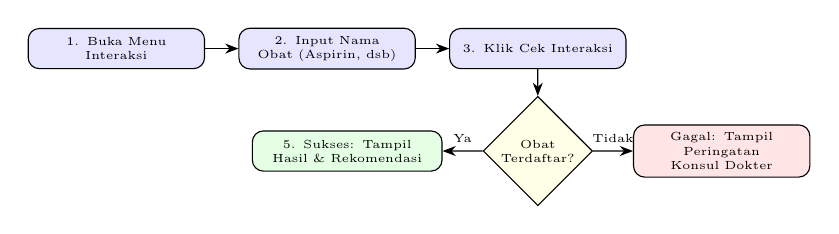
\begin{tikzpicture}[auto, >=Stealth, scale=0.85, every node/.style={transform shape},
        block/.style={rectangle, draw, fill=blue!10, text width=2.4cm, align=center, rounded corners, minimum height=0.6cm, font=\tiny},
        decision/.style={diamond, draw, fill=yellow!10, text width=1.3cm, align=center, inner sep=0pt, font=\tiny},
        err/.style={rectangle, draw, fill=red!10, text width=2.4cm, align=center, rounded corners, minimum height=0.6cm, font=\tiny},
        succ/.style={rectangle, draw, fill=green!10, text width=2.6cm, align=center, rounded corners, minimum height=0.6cm, font=\tiny}]
        
        \node (n1) [block] {1. Buka Menu Interaksi};
        \node (n2) [block, right=0.5cm of n1] {2. Input Nama Obat (Aspirin, dsb)};
        \node (n3) [block, right=0.5cm of n2] {3. Klik Cek Interaksi};
        \node (n4) [decision, below=0.4cm of n3] {Obat Terdaftar?};
        \node (n5) [succ, left=0.6cm of n4] {5. Sukses: Tampil Hasil \& Rekomendasi};
        \node (n6) [err, right=0.6cm of n4] {Gagal: Tampil Peringatan Konsul Dokter};
        
        \draw[->] (n1) -- (n2);
        \draw[->] (n2) -- (n3);
        \draw[->] (n3) -- (n4);
        \draw[->] (n4) -- node[above] {\tiny Ya} (n5);
        \draw[->] (n4) -- node[above] {\tiny Tidak} (n6);
    \end{tikzpicture}
\end{frame}

% --- SLIDE: USE CASE SCENARIO #6 ---
\begin{frame}{Use Case: Chat dengan Asisten AI (Obibi)}
    \centering
    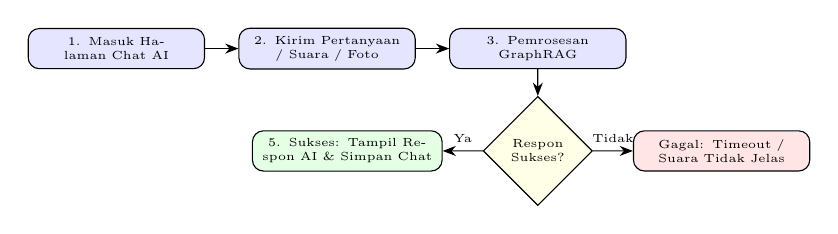
\begin{tikzpicture}[auto, >=Stealth, scale=0.85, every node/.style={transform shape},
        block/.style={rectangle, draw, fill=blue!10, text width=2.4cm, align=center, rounded corners, minimum height=0.6cm, font=\tiny},
        decision/.style={diamond, draw, fill=yellow!10, text width=1.3cm, align=center, inner sep=0pt, font=\tiny},
        err/.style={rectangle, draw, fill=red!10, text width=2.4cm, align=center, rounded corners, minimum height=0.6cm, font=\tiny},
        succ/.style={rectangle, draw, fill=green!10, text width=2.6cm, align=center, rounded corners, minimum height=0.6cm, font=\tiny}]
        
        \node (n1) [block] {1. Masuk Halaman Chat AI};
        \node (n2) [block, right=0.5cm of n1] {2. Kirim Pertanyaan / Suara / Foto};
        \node (n3) [block, right=0.5cm of n2] {3. Pemrosesan GraphRAG};
        \node (n4) [decision, below=0.4cm of n3] {Respon Sukses?};
        \node (n5) [succ, left=0.6cm of n4] {5. Sukses: Tampil Respon AI \& Simpan Chat};
        \node (n6) [err, right=0.6cm of n4] {Gagal: Timeout / Suara Tidak Jelas};
        
        \draw[->] (n1) -- (n2);
        \draw[->] (n2) -- (n3);
        \draw[->] (n3) -- (n4);
        \draw[->] (n4) -- node[above] {\tiny Ya} (n5);
        \draw[->] (n4) -- node[above] {\tiny Tidak} (n6);
    \end{tikzpicture}
\end{frame}

% --- SLIDE: SEQUENCE DIAGRAM ---
\begin{frame}{Sequence Diagram: Input Jadwal Obat}
    \centering
    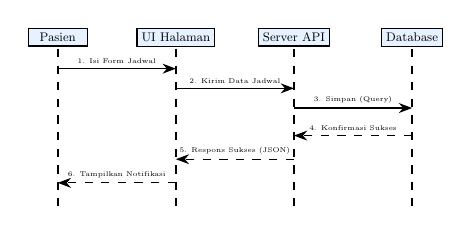
\begin{tikzpicture}[scale=0.5, every node/.style={transform shape}]
          % Lifelines
          \draw[thick, dashed] (0, 4) -- (0, 0);
          \draw[thick, dashed] (3, 4) -- (3, 0);
          \draw[thick, dashed] (6, 4) -- (6, 0);
          \draw[thick, dashed] (9, 4) -- (9, 0);

          % Objects
          \node[draw, fill=lightblue, minimum width=1.5cm] at (0, 4.3) {\small Pasien};
          \node[draw, fill=lightblue, minimum width=1.5cm] at (3, 4.3) {\small UI Halaman};
          \node[draw, fill=lightblue, minimum width=1.5cm] at (6, 4.3) {\small Server API};
          \node[draw, fill=lightblue, minimum width=1.5cm] at (9, 4.3) {\small Database};

          % Messages
          \draw[->, >=Stealth] (0, 3.5) -- node[above] {\tiny 1. Isi Form Jadwal} (3, 3.5);
          \draw[->, >=Stealth] (3, 3.0) -- node[above] {\tiny 2. Kirim Data Jadwal} (6, 3.0);
          \draw[->, >=Stealth] (6, 2.5) -- node[above] {\tiny 3. Simpan (Query)} (9, 2.5);
          
          \draw[->, >=Stealth, dashed] (9, 1.8) -- node[above] {\tiny 4. Konfirmasi Sukses} (6, 1.8);
          \draw[->, >=Stealth, dashed] (6, 1.2) -- node[above] {\tiny 5. Respons Sukses (JSON)} (3, 1.2);
          \draw[->, >=Stealth, dashed] (3, 0.6) -- node[above] {\tiny 6. Tampilkan Notifikasi} (0, 0.6);
    \end{tikzpicture}
    \begin{flushright}
        \tiny{\textit{Sumber: DPPL Aplikasi Obibi}}
    \end{flushright}
\end{frame}

% ======================================================================
% BAGIAN 4: PENGUJIAN PERANGKAT LUNAK (DUPL)
% ======================================================================
\section{Pengujian Perangkat Lunak}

% --- SLIDE: STRATEGI PENGUJIAN ---
\begin{frame}{Strategi \& Metode Pengujian}
    \begin{itemize}
        \item \textbf{Black-Box Testing}: Menguji fungsionalitas tanpa melihat kode internal.
        \item \textbf{Boundary Value Analysis (BVA)}: Validasi input ekstrem (format waktu, input kosong).
        \item \textbf{User Acceptance Testing (UAT)}: Melibatkan \textit{end-user} eksternal untuk memastikan kemudahan penggunaan.
    \end{itemize}
    \vspace{0.5cm}
    \begin{table}[]
    \small
    \begin{tabular}{|c|c|c|}
        \hline
        \textbf{Use Case} & \textbf{PIC} & \textbf{Jadwal} \\
        \hline
        Login & Ravi Adi Prakoso & 28 Mei 2026 \\
        Register & Muhammad Ahsan Raziq & 28 Mei 2026 \\
        Chatbot & Najla Tsabita & 28 Mei 2026 \\
        Input Obat & Revalina Rasyidin & 28 Mei 2026 \\
        Input Jadwal Obat & Ravi Adi Prakoso & 28 Mei 2026 \\
        \hline
    \end{tabular}
    \end{table}
\end{frame}

% --- SLIDE: HASIL PENGUJIAN ---
\begin{frame}{Hasil Pengujian Fungsional}
    \begin{table}[]
    \tiny
    \begin{tabular}{|c|c|c|c|}
        \hline
        \textbf{ID DUPL} & \textbf{Use Case} & \textbf{Skenario} & \textbf{Status} \\
        \hline
        DUPL-LOGIN-01 & Login & Login Berhasil & ✓ Valid \\
        DUPL-LOGIN-02 & Login & Login Gagal karena Internet & ✓ Valid \\
        DUPL-REGISTER-01 & Register & Register Berhasil & ✓ Valid \\
        DUPL-REGISTER-02 & Register & Register Gagal karena Internet & ✓ Valid \\
        DUPL-OBAT-01 & Kelola Obat & Input Data Obat Berhasil & ✓ Valid \\
        DUPL-OBAT-02 & Kelola Obat & Validasi Nama Obat Kosong & ✓ Valid \\
        DUPL-OBAT-03 & Kelola Obat & Hapus Data Obat Berhasil & ✓ Valid \\
        DUPL-INTERAKSI-01 & Cek Interaksi & Interaksi Obat Valid & ✓ Valid \\
        DUPL-INTERAKSI-02 & Cek Interaksi & Obat Tidak Ditemukan & ✓ Valid \\
        DUPL-INTERAKSI-03 & Cek Interaksi & Input Kosong & ✓ Valid \\
        DUPL-JADWAL-01 & Input Jadwal & Tambah Jadwal Berhasil & ✓ Valid \\
        DUPL-JADWAL-02 & Input Jadwal & Validasi Format Waktu & ✓ Valid \\
        DUPL-JADWAL-03 & Input Jadwal & Database Gagal Simpan & ✓ Valid \\
        \hline
    \end{tabular}
    \end{table}
    \vspace{0.3cm}
    \begin{block}{Kesimpulan}
        Semua butir uji dinyatakan \textbf{lolos} (\textit{All Clear}).
    \end{block}
\end{frame}

% --- SLIDE: MATRIKS PENGUJIAN TERHADAP REQUIREMENT ---
\begin{frame}{Matriks Pengujian terhadap FR}
    \begin{table}[]
    \begin{tabular}{|c|c|p{0.5\textwidth}|}
        \hline
        \textbf{Kode FR} & \textbf{Functional Requirement} & \textbf{ID DUPL} \\
        \hline
        FR-01 & Autentikasi Pengguna & DUPL-LOGIN-01, DUPL-LOGIN-02, DUPL-REGISTER-01, DUPL-REGISTER-02 \\
        FR-02 & Manajemen Data Obat & DUPL-OBAT-01 s.d. 03 \\
        FR-03 & Penjadwalan Konsumsi Obat & DUPL-JADWAL-01 s.d. 03 \\
        FR-10 & Deteksi Interaksi Antarobat & DUPL-INTERAKSI-01 s.d. 03 \\
        \hline
    \end{tabular}
    \end{table}
    \vspace{0.5cm}
    \begin{flushright}
        \tiny{\textit{Sumber: DUPL Aplikasi Obibi}}
    \end{flushright}
\end{frame}

% ======================================================================
% BAGIAN 5: KESIMPULAN
% ======================================================================
\section{Kesimpulan}

% --- SLIDE: KESIMPULAN ---
\begin{frame}{Kesimpulan}
    \begin{itemize}
        \item Aplikasi Obibi telah berhasil dirancang dan diuji sesuai dengan kebutuhan fungsional dan non-fungsional.
        \item Fitur utama (Login, Register, Cek Interaksi Obat, Input Jadwal) berfungsi dengan baik dan lolos pengujian.
        \item Sistem dibangun dengan arsitektur yang modular dan skalabel, siap untuk dikembangkan lebih lanjut.
        \item Pengujian \textit{User Acceptance} menunjukkan bahwa aplikasi ini \textbf{ramah pengguna} dan sesuai untuk target audiens (lansia dan penyandang disabilitas).
    \end{itemize}
    \vspace{0.5cm}
    \begin{block}{Rekomendasi}
        Pengembangan lebih lanjut pada fitur \textit{delighter} (AI Chatbot, Voice Command) dan integrasi dengan sistem eksternal.
    \end{block}
\end{frame}

% --- SLIDE: TERIMA KASIH ---
\begin{frame}
    \begin{center}
        \Huge{\textbf{TERIMA KASIH}}
        
        \vspace{0.5cm}
        \Large{Ada pertanyaan?}
        
        \vspace{1cm}
        \small{Dipersembahkan oleh:}
        
        \normalsize{Najla Tsabita Afiyah (103012400305)}
        
        \normalsize{Revalina Rasyidin (103012400156)}
        
        \normalsize{Ravi Adi Prakoso (103012430058)}
        
        \normalsize{Muhammad Ahsan Raziq Sulthany (103012430067)}
    \end{center}
\end{frame}

% ======================================================================
% LAMPIRAN: SCREENSHOT HASIL PENGUJIAN
% ======================================================================
\appendix
\section{Lampiran}

% --- SLIDE: SCREENSHOT PENGUJIAN ---
\begin{frame}{Lampiran: Screenshot Pengujian}
    \begin{columns}[T]
        \column{0.5\textwidth}
        \textbf{Login Sukses}
        \centering
        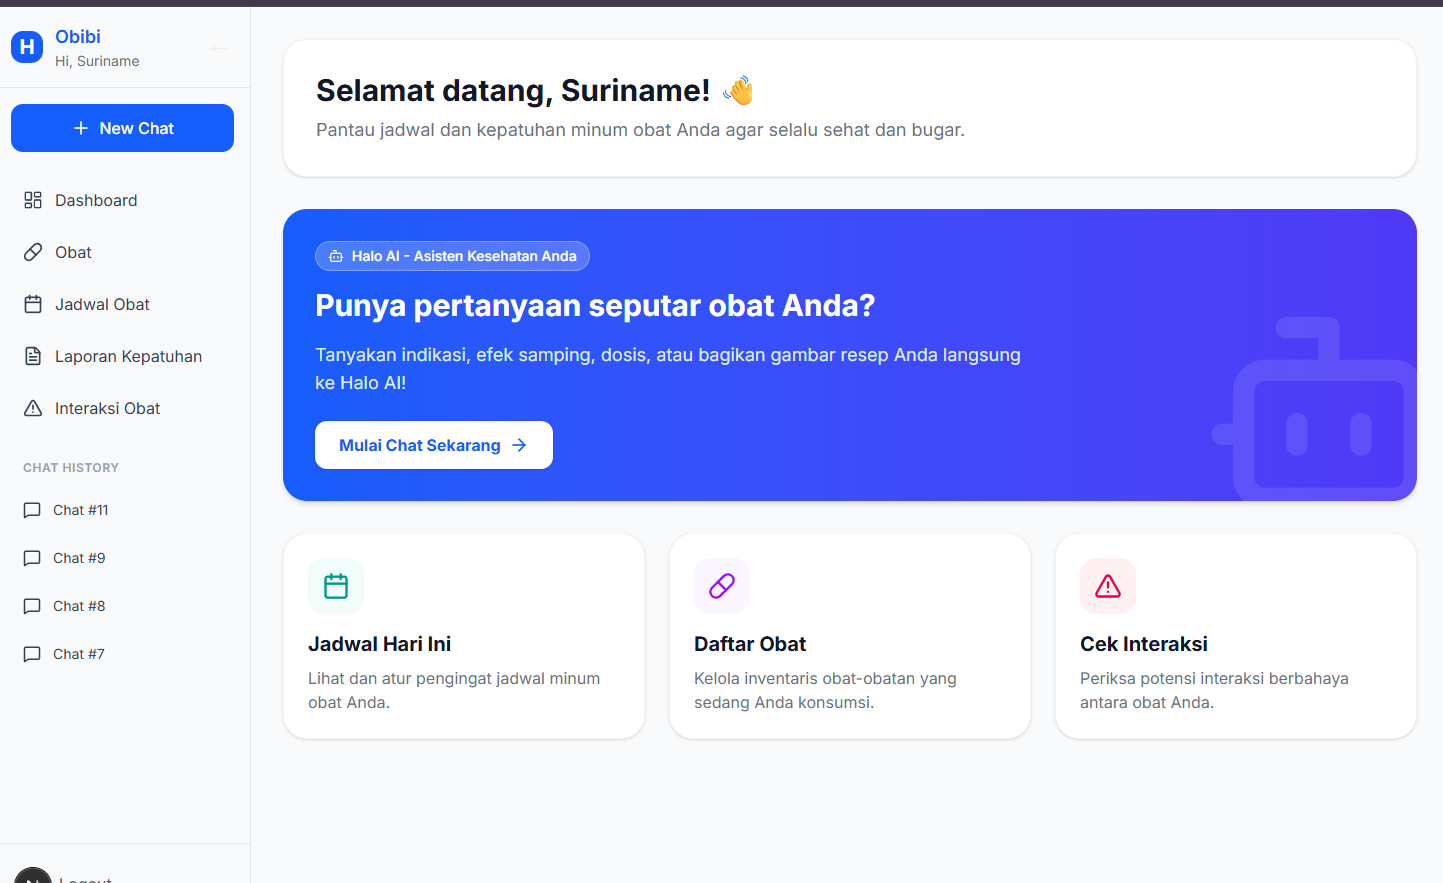
\includegraphics[width=0.65\textwidth]{loginberhasil.png}
        
        \column{0.5\textwidth}
        \textbf{Register Sukses}
        \centering
        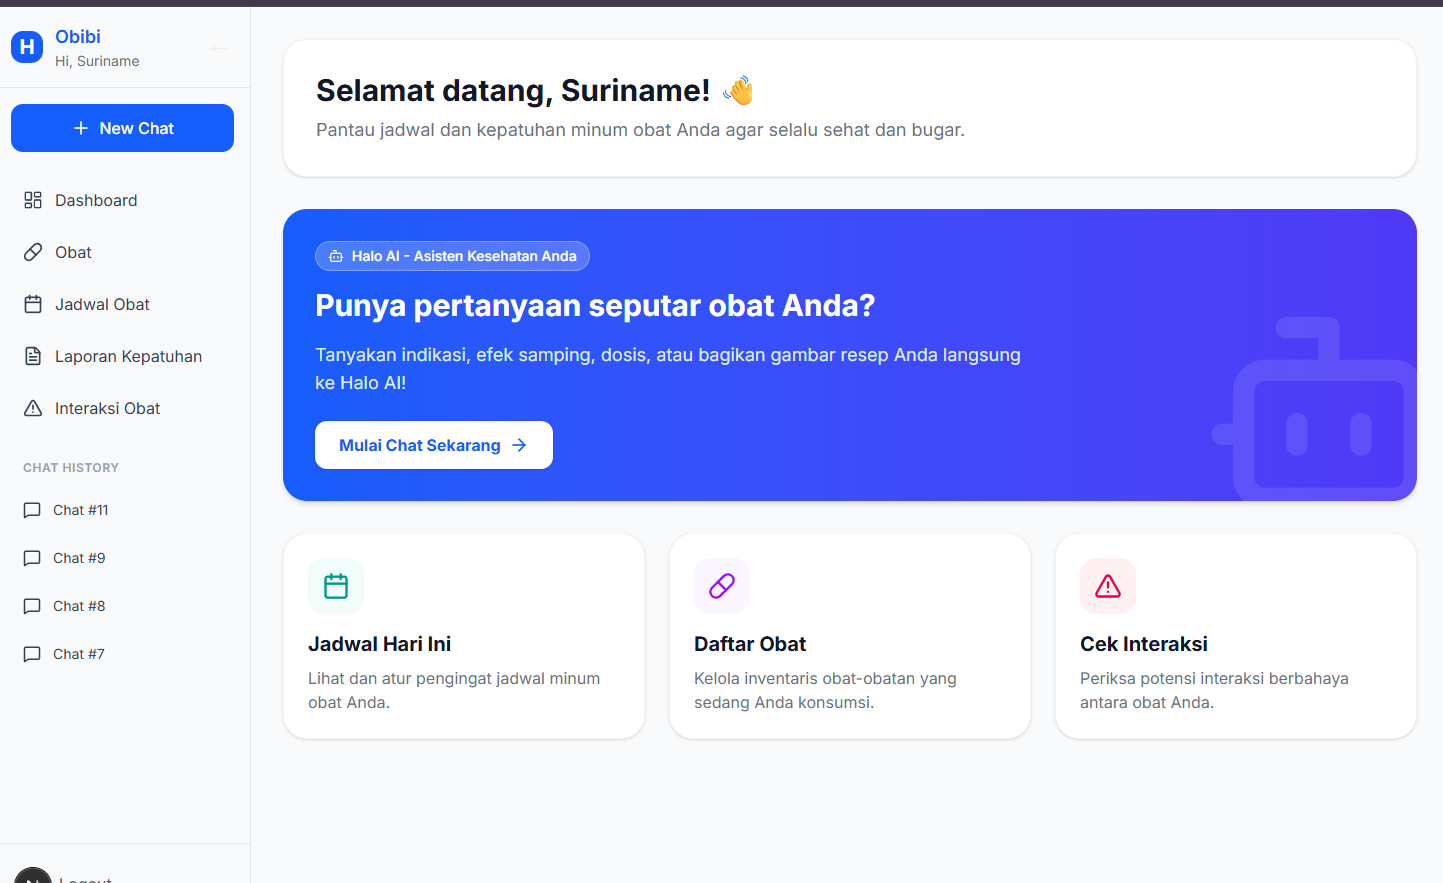
\includegraphics[width=0.65\textwidth]{registerberhasil.png}
    \end{columns}
    \begin{flushright}
        \tiny{\textit{Sumber: DUPL Aplikasi Obibi}}
    \end{flushright}
\end{frame}

% --- SLIDE: SCREENSHOT PENGUJIAN (2) ---
\begin{frame}{Lampiran: Screenshot Pengujian (2)}
    \begin{columns}[T]
        \column{0.5\textwidth}
        \textbf{Error Koneksi}
        \centering
        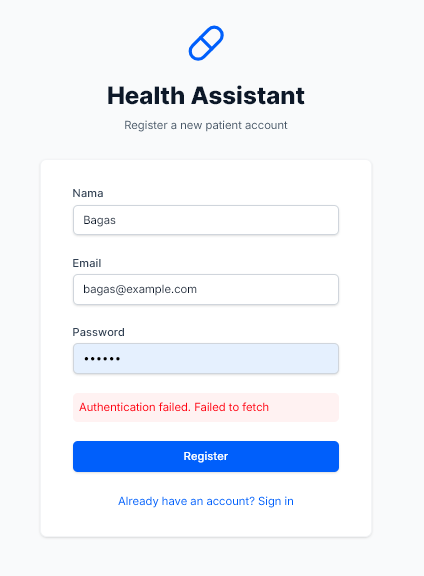
\includegraphics[width=0.65\textwidth]{regErrornointernet.png}
        
        \column{0.5\textwidth}
        \textbf{Hasil Interaksi Obat}
        \centering
        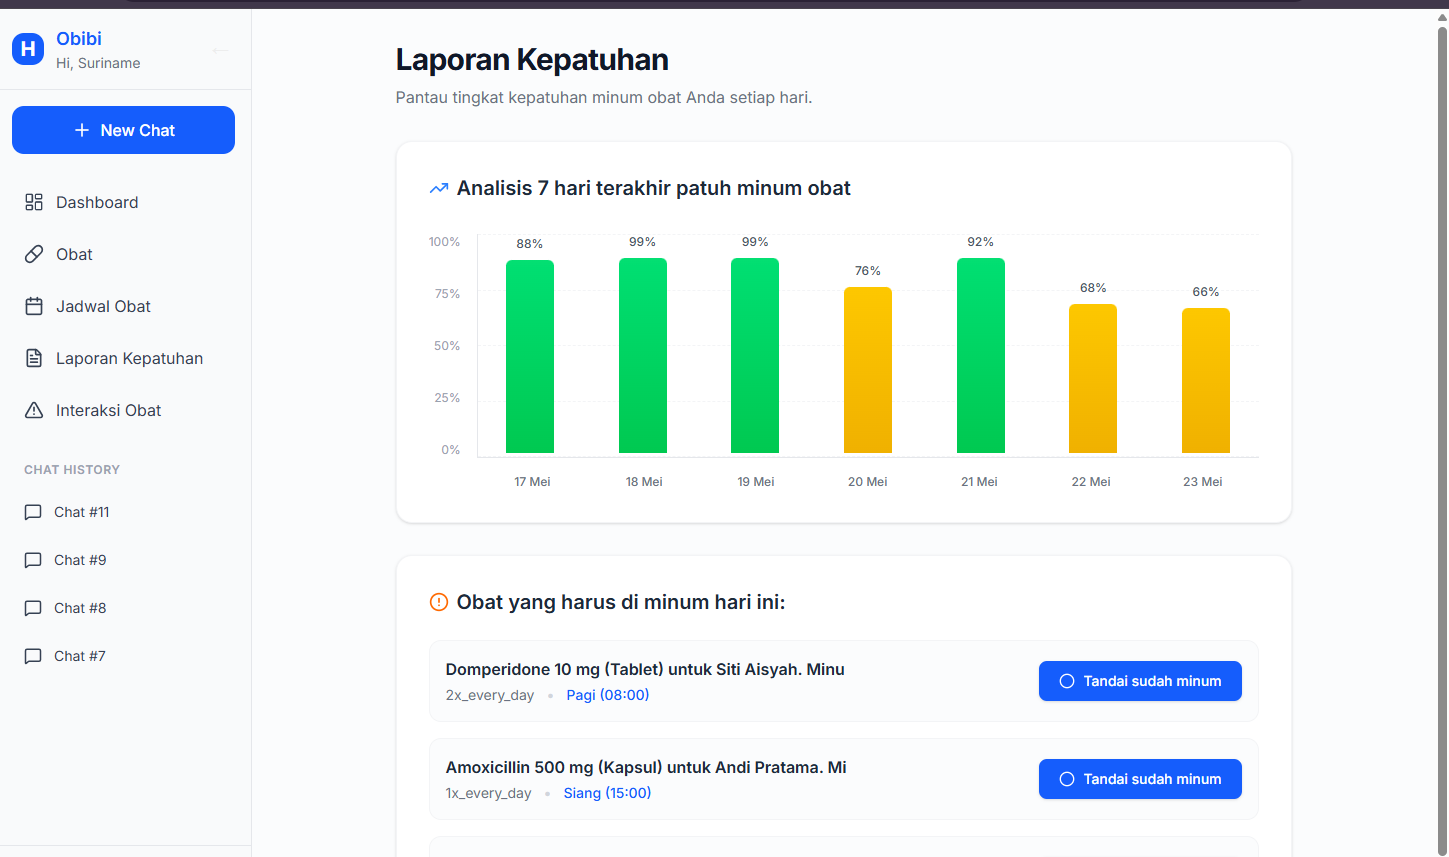
\includegraphics[width=0.65\textwidth]{laporankepatuhan.png}
    \end{columns}
\end{frame}

% --- SLIDE: SCREENSHOT PENGUJIAN (3) ---
\begin{frame}{Lampiran: Screenshot Pengujian (3)}
    \centering
    \textbf{Input Jadwal Obat}
    \vspace{0.2cm}
    
    \includegraphics[height=0.55\textheight, keepaspectratio]{input_obat.png}
    \begin{flushright}
        \tiny{\textit{Sumber: DUPL Aplikasi Obibi}}
    \end{flushright}
\end{frame}

% --- SLIDE: SCREENSHOT PENGUJIAN (4) ---
\begin{frame}{Lampiran: Screenshot Pengujian (4)}
    \centering
    \textbf{Kelola Data Obat}
    \vspace{0.2cm}
    
    \includegraphics[height=0.55\textheight, keepaspectratio]{kelola_obat.png}
    \begin{flushright}
        \tiny{\textit{Sumber: DUPL Aplikasi Obibi}}
    \end{flushright}
\end{frame}

\end{document}